\documentclass[tikz,png]{standalone}
\usepackage{unicode-math}
\usetikzlibrary{positioning}
\begin{document}
  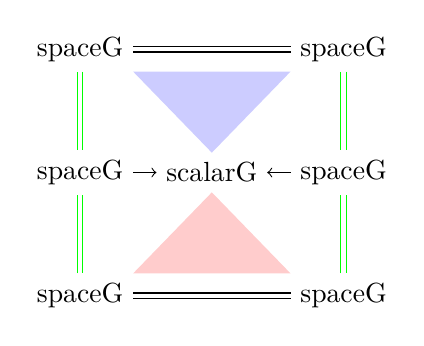
\begin{tikzpicture}
    % s₀
    \node (s) {scalarG};
    \node[left = of s.center] (s0l) {spaceG};
    \node[right = of s.center] (s0r) {spaceG};
    \draw[->] (s0l) -- (s);
    \draw[->] (s0r) -- (s);
    % r₁
    \node[above = of s0l] (r1l) {spaceG};
    \node[above = of s0r] (r1r) {spaceG};
    \draw[double equal sign distance] (r1l) -- (r1r);
    % r₀
    \node[below = of s0l] (r0l) {spaceG};
    \node[below = of s0r] (r0r) {spaceG};
    \draw[double equal sign distance] (r0l) -- (r0r);
    % forward cone
    \fill[fill=red!20] (r0l.north east) -- (s.south) -- (r0r.north west);
    % backward cone
    \fill[fill=blue!20] (r1l.south east) -- (s.north) -- (r1r.south west);
    % equalities between regular heights
    \draw[green,double equal sign distance] (r1l) -- (s0l);
    \draw[green,double equal sign distance] (r1r) -- (s0r);
    \draw[green,double equal sign distance] (r0l) -- (s0l);
    \draw[green,double equal sign distance] (r0r) -- (s0r);
  \end{tikzpicture}
\end{document}
